L'architettura di \textit{HDViz} è basata sul \glo{design architetturale} \glo{\textit{Model-View-ViewModel (MVVM)}}, derivato dal più comune \glo{Model-View-Controller (MVC)}. 
È stato scelto MVVM per i seguenti motivi: 
\begin{itemize}
	\item Favorisce la separazione tra \glo{\textit{business logic}} e \glo{\textit{presentational logic}}, facendo comunicare \textit{Model} e \textit{View} solo attraverso il \textit{ViewModel};  
	\item Permette di non avere un unico controller con cui dover gestire tutta la \glo{\textit{application logic}}. Essa è infatti suddivisa nei vari componenti che compongono la vista, fornendo diversi vantaggi: 
	\begin{itemize}
		\item Minor numero di conflitti in fase di codifica (non si deve accedere a uno stesso file dove è contenuta tutta la logica);
		\item Performance migliori (viene renderizzato solo il componente che effettivamente subisce modifiche del proprio \glo{stato interno}).
	\end{itemize}
	\item Adatto per le web app la cui interfaccia utente è sviluppata con la libreria React.
\end{itemize}

La comunicazione tra \textit{View} e \textit{ViewModel} avviene attraverso un contesto (\glo{\textit{Context React}}) con il quale la vista è in grado di accedere e modificare il valore dei dati presenti nel \textit{ViewModel}, il quale contiene un'istanza del \textit{Model}. \\
L'utilizzo di un \textit{Context React} permette di non passare \glo{\textit{props}} in tutta la vista (da componente padre a componente figlio), evitando il possibile problema di dover attraversare tutta la gerarchia prima di raggiungere il componente che effettivamente le deve utilizzare.

\begin{figure}[hb]
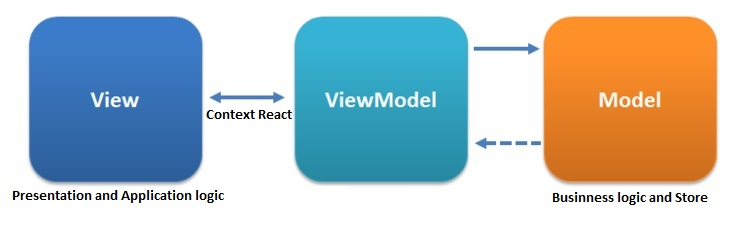
\includegraphics[width=15.8cm]{Extra/MVVMPattern}
\centering
\caption{Model-View-ViewModel (MVVM)}
\end{figure}